\documentclass[UTF8,12pt]{ctexart}
\usepackage{amsmath}
\usepackage{graphicx}
\usepackage{float}
\usepackage{geometry}
\usepackage{booktabs}
\usepackage[hidelinks]{hyperref}
\usepackage{listings}
\usepackage{xcolor}

% 设置代码样式
\lstset{
    basicstyle=\ttfamily\small,      % 字体
    keywordstyle=\color{blue},       % 关键字颜色
    commentstyle=\color{green!60},   % 注释颜色
    stringstyle=\color{red},         % 字符串颜色
    numbers=left,                    % 行号位置
    numberstyle=\tiny\color{gray},   % 行号样式
    breaklines=true,                 % 自动换行
    frame=single,                    % 边框
    captionpos=b                     % 标题位置
}

\setlength{\parindent}{2em} % 设置首行缩进

\title{《数据可视化》技术报告\\[0.3cm] \normalsize ——数据可视化的常规形式综述与在数据科学领域的部分实现}   % 标题
\author{姓名: 贺正泽\\学号: 2023302021155\\学院: 数学与统计学院}

\date{2026年5月10日}


\begin{document}    % begin和end标识出正文的范围

\maketitle   % 生成标题
\newpage
\tableofcontents   % 生成目录
\newpage

\section{引言}
数据可视化是将数据以图像的形式呈现出来，以便更好地理解、分析和传达信息的过程。随着大数据时代的到来，数据可视化在各个领域变得越来越重要。通过有效的数据可视化，我们可以揭示数据中的模式、趋势和关系，从而支持决策制定和科学研究。本报告将介绍数据可视化的常规形式及其应用，并且探讨数据科学领域的数据可视化。本报告将通过Springer检索``Data Science"相关文献，检索结果中 Subjects 栏目下的相关主题及对应文献数量，绘制横向条形图和文字云图，从而分析数据科学领域的研究热点,并且以机器学习中的 P-R曲线为例反映数据可视化在机器学习中的应用。


\section{常规可视化形式}

\subsection{线图}
线图是一种常见的连续型数据可视化方式，通常用于展示变量随时间或其他连续变量\textbf{变化的趋势}。在线图中，横轴一般表示时间、序号或\textbf{连续自变量}，纵轴表示观测值，通过折线连接各个数据点，从而反映整体变化趋势。本质上也可以通过密集的取点来近似连续数据的变化趋势从而绘制表达式或函数。

线图适用于时间序列数据分析，例如股票价格变化、气温变化、网站访问量变化以及商品销售额变化等。在数据分析过程中，线图可以帮助观察数据的上升、下降、周期性波动和异常变化。

例如，在机器学习模型训练过程中，可以使用线图展示模型损失函数值或准确率随训练轮数的变化趋势。如果损失函数随着训练轮数增加而逐渐下降，说明模型正在不断学习数据中的规律；如果验证集准确率在某一轮之后不再提升甚至下降，则可能说明模型出现了过拟合现象。

\subsection{数据分布图}
数据分布图主要用于展示数据的\textbf{分布特征和组成结构}，常见形式包括直方图、饼图、气泡图、箱线图和小提琴图等。

直方图通过将连续数据划分为若干区间，并统计每个区间中的样本数量，用于展示数值型变量的分布形态、集中趋势和离散程度。饼图通过扇形面积表示不同类别在总体中的占比，适合展示类别变量的组成结构。气泡图在散点图的基础上引入气泡大小这一视觉变量，可以同时展示多个变量之间的关系，例如用横轴、纵轴和气泡大小分别表示三个不同指标。箱线图通过最小值、下四分位数、中位数、上四分位数和最大值展示数据分布情况，并能够直观识别异常值。小提琴图结合了箱线图和密度图的特点，不仅可以展示数据的中位数和离散程度，还能够反映数据在不同取值区间的密集程度。

在数据科学中，数据分布图常用于探索性数据分析。例如，在建立预测模型之前，可以使用直方图查看特征变量是否近似服从正态分布，使用箱线图观察不同类别下数值变量的差异。如果某些变量存在严重偏态分布或极端异常值，则可能需要进行数据变换或异常值处理。


\subsection{离散数据图}
离散数据图主要用于展示\textbf{类别型变量}之间的数量关系，常见形式包括条形图、散点图等。

条形图适合比较不同类别之间的数量差异。例如，可以用条形图展示不同专业学生人数、不同地区销售额或不同商品类别的订单数量。散点图则适合展示两个变量之间的关系，但如果其中一个变量是类别型变量，也可以通过不同颜色或形状的点来区分不同类别，从而观察类别之间的关系。

在数据科学应用中，离散数据图常用于观察类别变量的分布情况。例如，在分类任务中，可以使用条形图观察不同类别样本的数量是否均衡。如果类别分布严重不平衡，则模型训练时可能需要采用重采样、类别权重调整等方法。


\subsection{极坐标图与等高线图}
极坐标图使用\textbf{角度和半径}表示数据，适合展示具有周期性或方向性的数据。例如，风向频率图、周期性销售变化图以及雷达图都可以看作极坐标思想的应用。在绘制极坐标图时，数据在极坐标图与笛卡尔坐标系之间的转换需要进行坐标变换，具体公式如下：
\[
\begin{cases}
x = \rho \cdot \cos(\theta) \\[4pt]
y = \rho \cdot \sin(\theta)
\end{cases}
\qquad\Longleftrightarrow\qquad
\begin{cases}
\rho = \sqrt{x^2 + y^2} \\[4pt]
\theta = \operatorname{atan2}(y, x)
\end{cases}
\]
其中，$\rho$ 表示半径，$\theta$ 表示角度，$x$ 和 $y$ 分别表示笛卡尔坐标系中的横纵坐标。

等高线图通常用于展示二维平面上某一连续变量的变化情况。它通过连接函数值相同的点形成等高线，可以反映变量在空间上的变化趋势。在数学建模和机器学习中，等高线图常用于展示损失函数曲面、概率密度分布或地形高度变化。

例如，在机器学习模型优化过程中，可以用等高线图展示不同参数组合下模型损失函数的变化情况，从而帮助理解梯度下降算法的优化路径。


\subsection{向量场}
向量场是一种用于展示\textbf{带有方向和大小的数据}的可视化形式。图中的每一个箭头通常表示某一点处向量的方向和强度。向量场广泛应用于物理、气象、流体力学以及动态系统分析中。

在数据科学中，向量场也具有一定应用价值。例如，在降维和优化算法中，可以使用向量场展示数据点移动方向或梯度变化方向。在机器学习中，梯度下降算法的参数更新过程也可以通过向量场进行直观表示。

向量场的优势在于能够同时表达方向和大小两个信息维度，使得观察者可以更好地理解动态变化过程。


\section{数据科学领域的数据可视化}

\subsection{Data Science相关文献的检索文字云图分析}
为了分析数据科学与大数据技术领域的研究主题分布，本文以``Data Science and Big Data Technology"为关键词，在 Springer 数据库中进行检索，并提取检索结果中 Subjects 栏目下的相关主题及对应文献数量。Subjects 是 Springer 根据文献内容归纳出的主题分类，因此能够在一定程度上反映该领域的研究热点和应用方向。得到的主题分类数据如下表所示:

\begin{table}[H]
\centering
\caption{Springer中Data Science and Big Data Technology相关主题统计}
\begin{tabular}{llr}
\toprule
序号 & 主题 & 文献数量 \\
\midrule
1 & Artificial intelligence & 9384 \\
2 & Machine learning & 7921 \\
3 & Computational intelligence & 6170 \\
4 & Big data & 5983 \\
5 & Educational research & 5403 \\
6 & Technological innovation & 4963 \\
7 & Knowledge and innovation & 4685 \\
8 & Internet of things & 4346 \\
9 & Data analysis and big data & 4082 \\
10 & Data mining & 4039 \\
11 & Cloud computing & 3904 \\
12 & Smart infrastructure & 3816 \\
13 & Knowledge based systems & 3616 \\
14 & Internet of things applications in smart environments & 3558 \\
15 & Philosophy of artificial intelligence & 3523 \\
16 & Education science & 3518 \\
\bottomrule
\end{tabular}
\end{table}


本文选取文献数量较多的前16个主题作为分析对象，同时剔除搜索关键词``Data Science and Big Data Technology"中已含的文本，将主题名称及对应数量整理为结构化数据。随后，利用 MATLAB 绘制横向条形图和文字云图。横向条形图能够清晰比较不同主题对应的文献数量差异，而文字云图则通过字体大小直观展示主题的重要程度。

\begin{figure}[H]
    \centering
    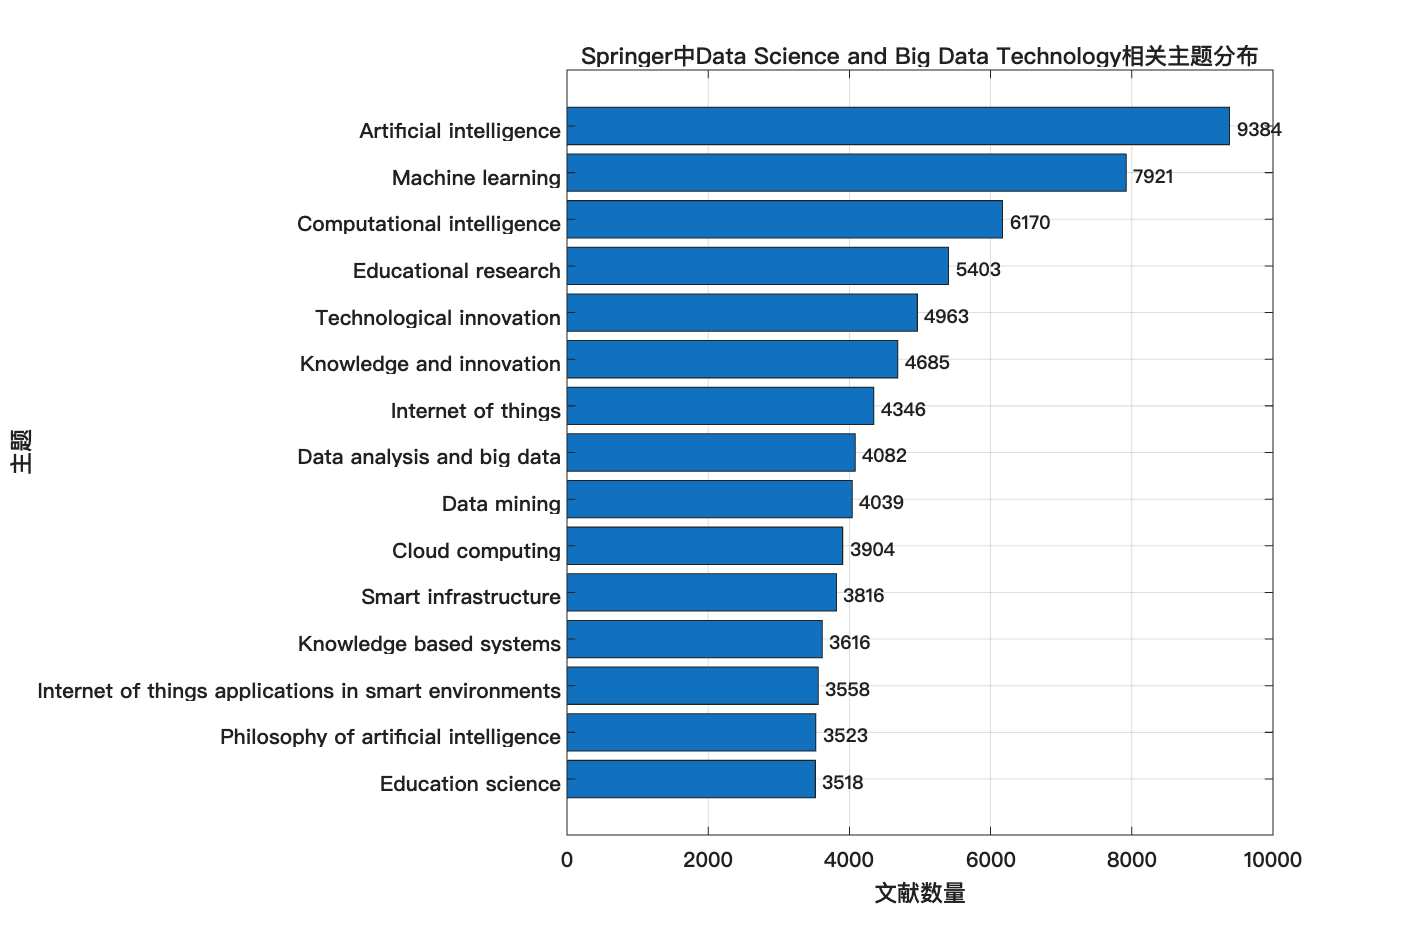
\includegraphics[width=1.0\textwidth]{subject_bar.png}
    \caption{Springer中Data Science and Big Data Technology相关主题分布}
\end{figure}

\begin{figure}[H]
    \centering
    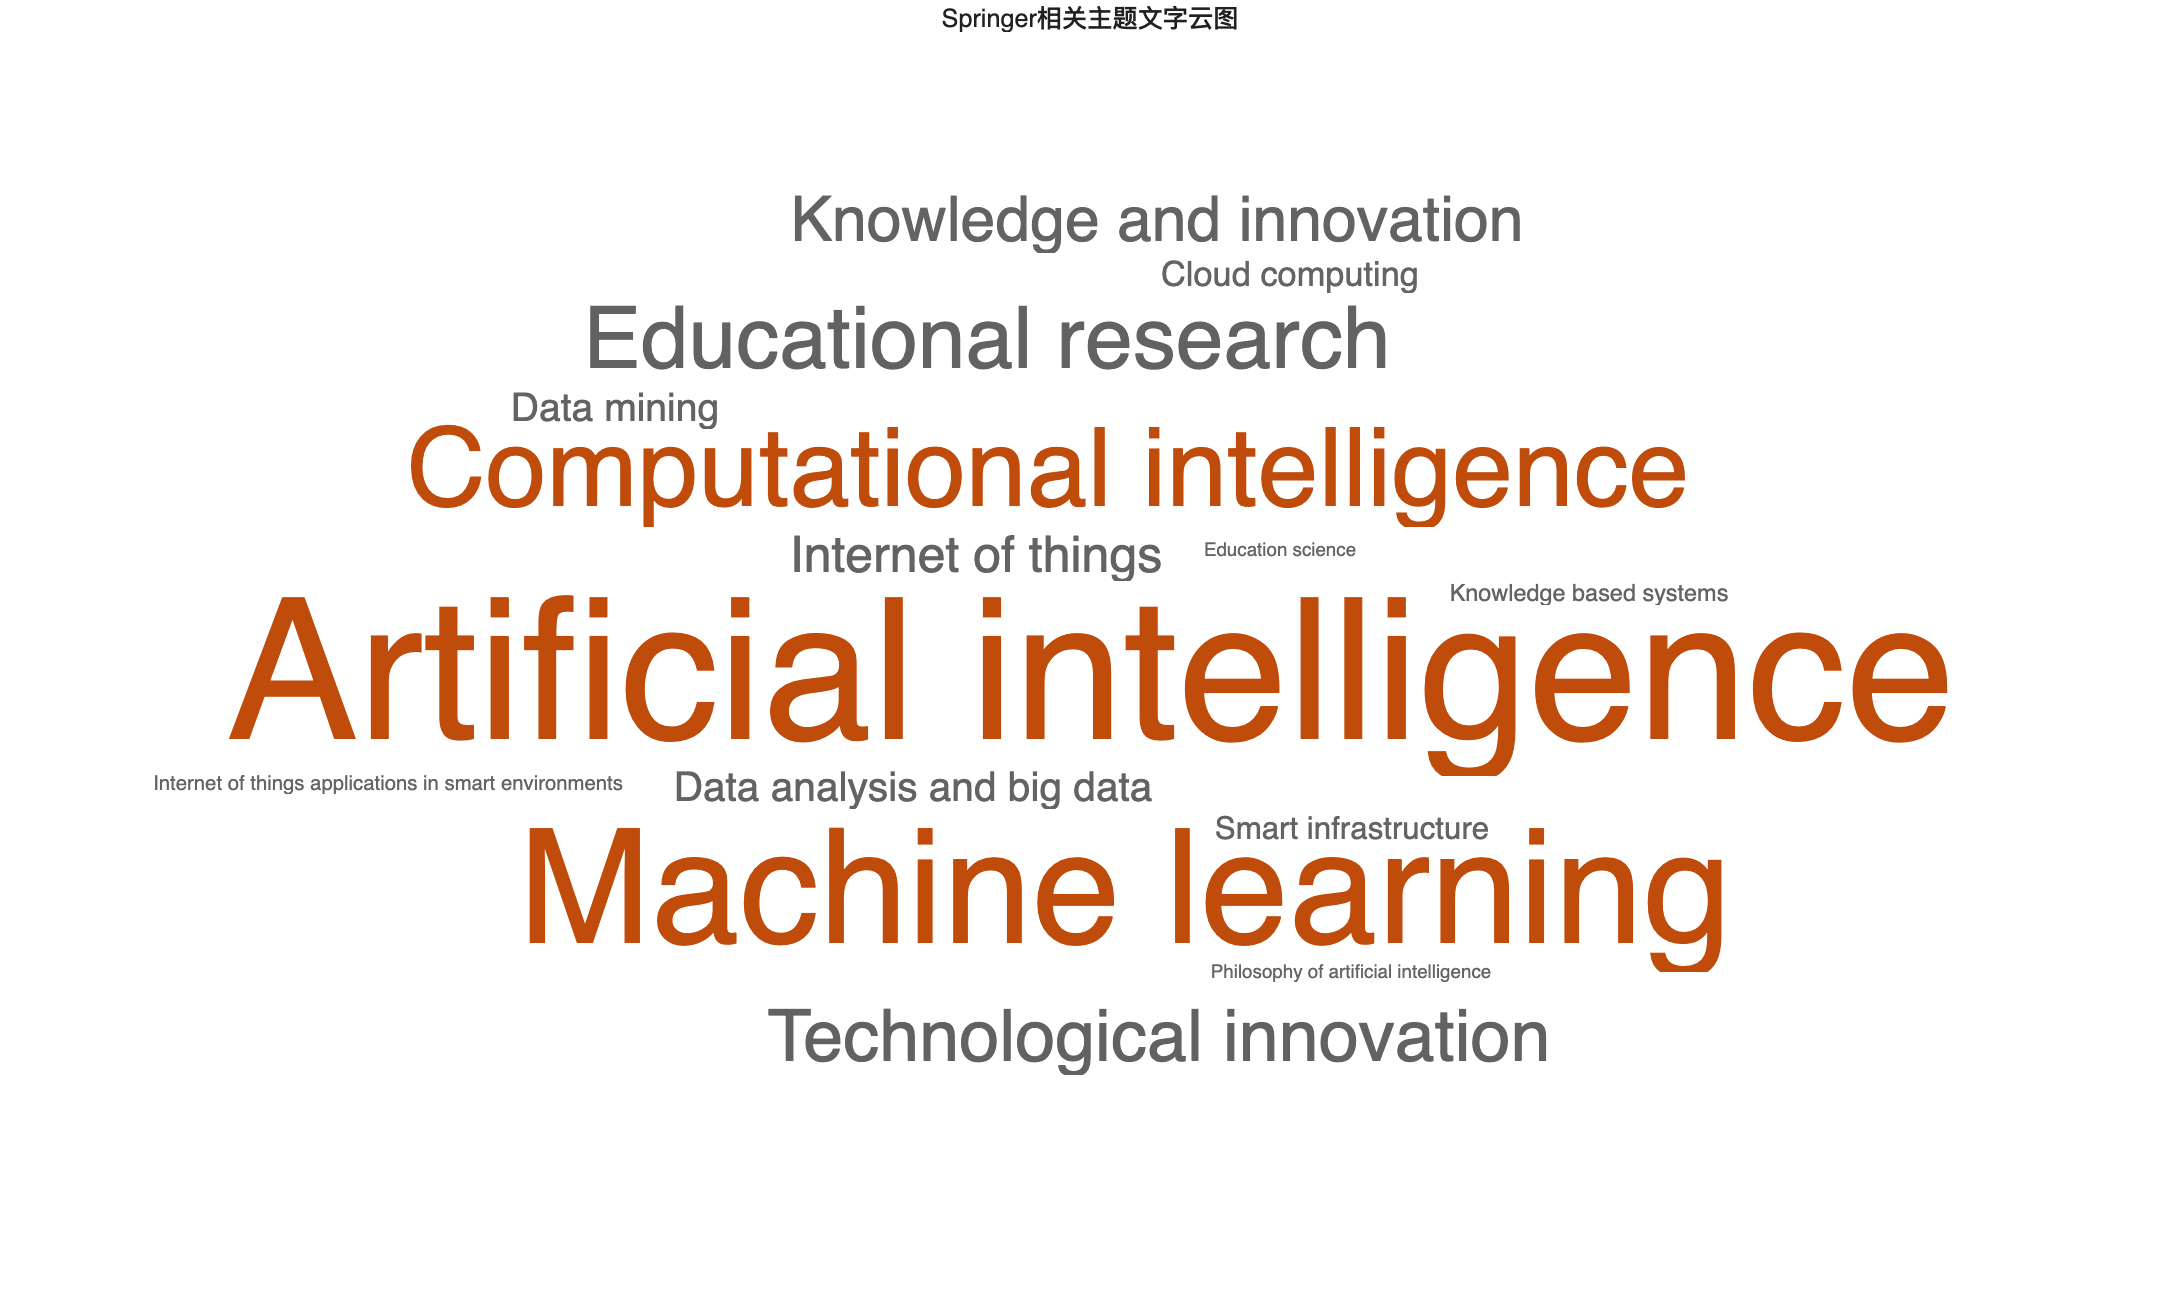
\includegraphics[width=1.0\textwidth]{subject_wordcloud.png}
    \caption{Springer中Data Science and Big Data Technology相关主题文字云图}
\end{figure}

从图中可以看出，``Artificial intelligence"对应的文献数量最多，达到9384篇；其次是``Machine learning"，数量为7921篇。这说明人工智能和机器学习是数据科学与大数据技术领域中最核心的研究方向。数据科学的发展与智能算法密切相关，机器学习方法为数据建模、预测分析、模式识别和自动决策提供了重要技术支撑。

``Computational intelligence"、``Knowledge based systems"和``Philosophy of artificial intelligence"等主题也具有较高频次，说明该领域不仅关注具体算法和模型，也关注智能系统、知识表示以及人工智能相关的理论与社会问题。

此外，``Data analysis and big data"、``Data mining" 和 ``Cloud computing" 等主题的出现频次也较高。这表明数据科学与大数据技术密切相关，其研究对象通常具有数据规模大、类型复杂、处理速度要求高等特点。云计算为大规模数据存储和计算提供了基础设施，而数据挖掘和数据分析方法则用于从海量数据中提取有价值的信息。

从应用场景来看，``Internet of things"、``Smart infrastructure" 和 ``Internet of things applications in smart environments" 等主题的出现说明数据科学与物联网、智慧环境和智能基础设施建设之间存在紧密联系。随着传感器、智能设备和网络系统的发展，来自现实世界的大量数据可以被采集、分析和利用，从而支持智慧城市、智能交通和智能环境管理等应用。

文字云图进一步直观展示了各主题的重要程度。字号较大的``Artificial intelligence"、``Machine learning"和``Computational intelligence"表明，人工智能、机器学习和计算智能是该领域的核心关键词。整体来看，数据科学与大数据技术并不是单一技术方向，而是融合了人工智能、机器学习、云计算、数据挖掘、物联网和教育应用等多个方向的交叉学科。


\subsection{机器学习中的P-R曲线}
在机器学习分类任务中，模型评价是非常重要的环节。对于二分类问题，常见的评价指标包括准确率、查准率、查全率、F1值、ROC曲线和P-R曲线等。其中，P-R曲线是查准率-查全率曲线，特别适用于类别不平衡的数据集。

查准率表示模型预测为正类的样本中，真正为正类的比例，其公式为：

\[
Precision = \frac{TP}{TP + FP}
\]

查全率表示所有真实正类样本中，被模型正确识别出来的比例，其公式为：

\[
Recall = \frac{TP}{TP + FN}
\]

其中，$TP$ 表示真正例，$FP$ 表示假正例，$FN$ 表示假负例。

P-R曲线以查全率为横轴、查准率为纵轴，通过改变分类阈值，可以得到不同的查准率和查全率组合。一般来说，模型性能越好，PR曲线越靠近右上角。在类别不平衡问题中，例如欺诈检测、疾病诊断、垃圾邮件识别等任务，负类样本往往远多于正类样本，此时准确率可能具有误导性，而PR曲线能够更好地反映模型对少数类样本的识别能力。以下图为例，展示了一个机器学习分类模型的PR曲线示意图。

\begin{figure}[H]
    \centering
    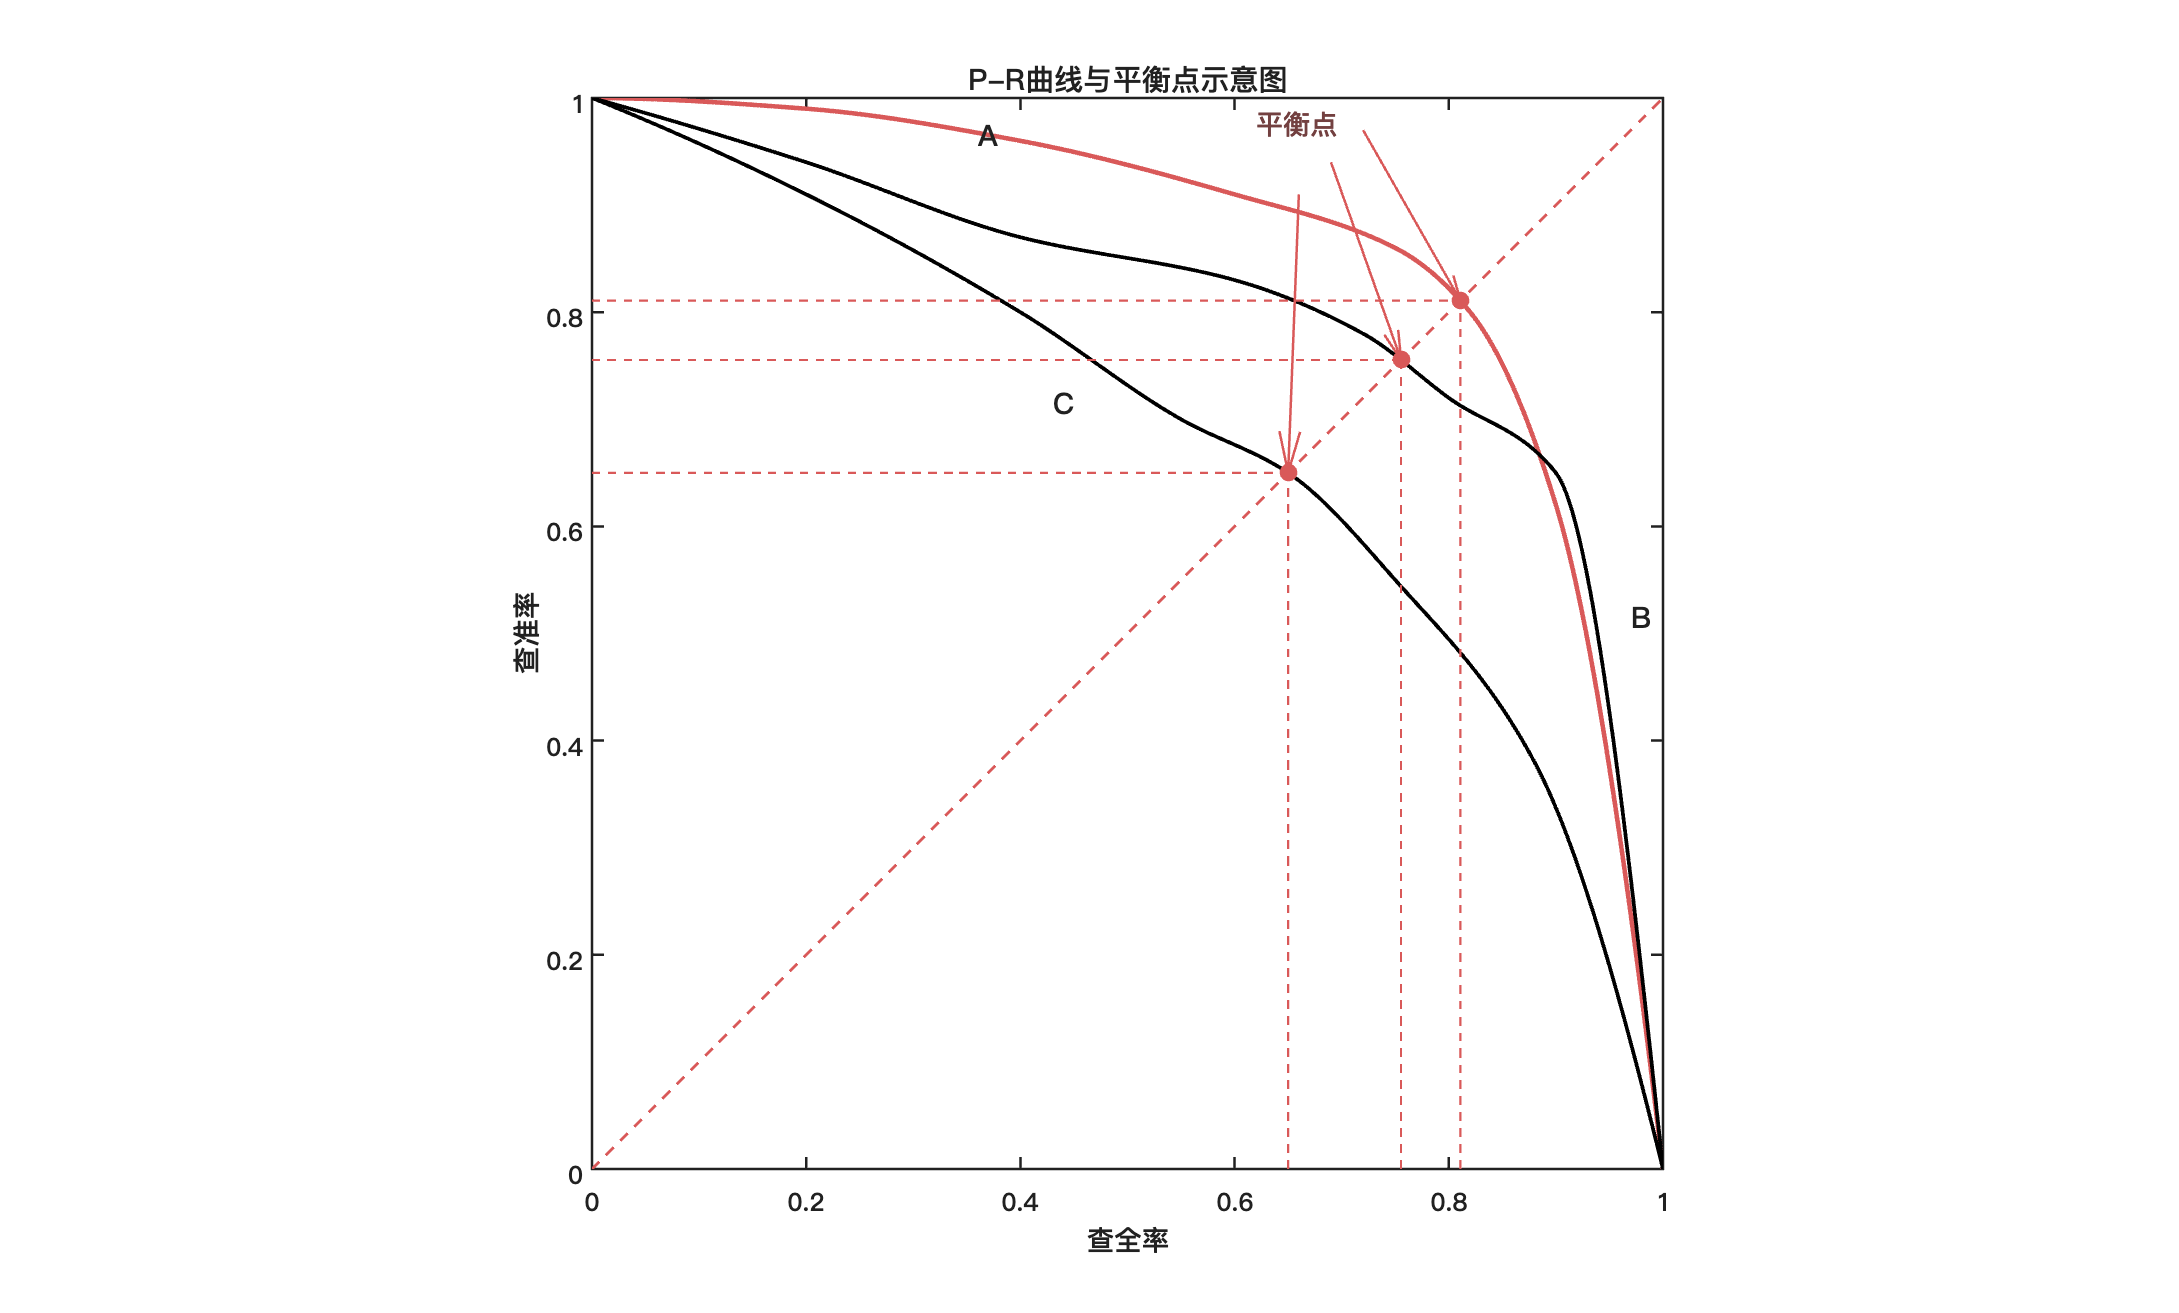
\includegraphics[width=1.0\textwidth]{PR_plot.png}
    \caption{机器学习分类模型的PR曲线示意图}
\end{figure}

在进⾏⽐较时， 若⼀个学习器的P-R曲线被另⼀个学习器的曲线完全“包住”，则可断⾔后者的性能优于前者，例如图3中学习器A的性能优于学习器C；如果两个学习器的P-R曲线发⽣了交叉，例如图3中的A与B，则难以⼀般性地断⾔两者敦优孰劣，只能在具体的查准率或查全率条件下进⾏⽐较。例如比较在查准率等于查全率时学习器的平衡点。

在一些应用中，对查准率和查全率的重视程度有所不同。例如在商品推荐系统中，为了尽可能少打扰用户，更希望推荐内容确是用户感兴趣的，此时查准率更重要；而在逃犯信息检索系统中，更希望尽可能少漏掉逃犯，此时查全率更重要。P-R曲线能够更清楚地展示模型在不同场景下对查准率和查全率之间的权衡关系。

P-R曲线体现了数据科学可视化的专业特点：它不仅仅是展示数据本身，还用于解释模型性能和辅助模型选择。通过可视化曲线，研究者可以根据实际任务需求选择合适的分类阈值。

\section{可视化的源代码展示}
\subsection{横向条形图的MATLAB代码示例}
以下是使用MATLAB绘制横向条形图的示例代码：
\begin{lstlisting}
clc; clear; close all;

subjects = {
    'Artificial intelligence'
    'Machine learning'
    'Computational intelligence'
    'Educational research'
    'Technological innovation'
    'Knowledge and innovation'
    'Internet of things'
    'Data analysis and big data'
    'Data mining'
    'Cloud computing'
    'Smart infrastructure'
    'Knowledge based systems'
    'Internet of things applications in smart environments'
    'Philosophy of artificial intelligence'
    'Education science'
};

counts = [9384 7921 6170 5403 4963 4685 4346 ...
          4082 4039 3904 3816 3616 3558 3523 3518];

% 为了让数量最多的主题显示在最上方，需要反转顺序
subjects_rev = flip(subjects);
counts_rev = flip(counts);

figure;
barh(counts_rev);

set(gca, 'YTick', 1:length(subjects_rev));
set(gca, 'YTickLabel', subjects_rev);
xlabel('文献数量');
ylabel('主题');
title('Springer中Data Science and Big Data Technology相关主题分布');
grid on;

% 在柱子右侧标注数量
for i = 1:length(counts_rev)
    text(counts_rev(i) + 100, i, num2str(counts_rev(i)), ...
        'VerticalAlignment', 'middle', 'FontSize', 9);
end

set(gca, 'FontSize', 10);
set(gcf, 'Position', [100 100 900 600]);
\end{lstlisting}

\subsection{文字云图的MATLAB代码示例}
以下是使用MATLAB绘制文字云图的示例代码：
\begin{lstlisting}
clc; clear; close all;

subjects = [
    "Artificial intelligence"
    "Machine learning"
    "Computational intelligence"
    "Educational research"
    "Technological innovation"
    "Knowledge and innovation"
    "Internet of things"
    "Data analysis and big data"
    "Data mining"
    "Cloud computing"
    "Smart infrastructure"
    "Knowledge based systems"
    "Internet of things applications in smart environments"
    "Philosophy of artificial intelligence"
    "Education science"
];

counts = [9384 7921 6170 5403 4963 4685 4346 ...
          4082 4039 3904 3816 3616 3558 3523 3518];

figure;
wordcloud(subjects, counts);
title('Springer相关主题文字云图');
\end{lstlisting}

\subsection{P-R曲线的MATLAB代码示例}
以下是使用MATLAB绘制P-R曲线的示例代码：
\begin{lstlisting}
clc; clear; close all;

% 设置中文字体
set(0,'defaultAxesFontName','SimSun');
set(0,'defaultTextFontName','SimSun');

% 横轴：查全率 Recall
x = linspace(0,1,500);

% 构造三条 P-R 曲线的控制点
xA = [0 0.2 0.4 0.6 0.75 0.82 0.9 1.0];
yA = [1 0.99 0.96 0.91 0.86 0.80 0.62 0];

xB = [0 0.2 0.4 0.6 0.72 0.80 0.9 1.0];
yB = [1 0.94 0.87 0.83 0.78 0.72 0.65 0];

xC = [0 0.2 0.4 0.55 0.65 0.75 0.88 1.0];
yC = [1 0.91 0.80 0.70 0.65 0.55 0.38 0];

% 使用 pchip 插值得到平滑曲线
YA = interp1(xA, yA, x, 'pchip');
YB = interp1(xB, yB, x, 'pchip');
YC = interp1(xC, yC, x, 'pchip');

YA = max(min(YA,1),0);
YB = max(min(YB,1),0);
YC = max(min(YC,1),0);

% -------------------------------------------------
% 求平衡点：即 P-R 曲线与 y = x 的交点
% -------------------------------------------------
fA = @(t) interp1(xA, yA, t, 'pchip') - t;
fB = @(t) interp1(xB, yB, t, 'pchip') - t;
fC = @(t) interp1(xC, yC, t, 'pchip') - t;

pxA = fzero(fA, [0 1]);
pxB = fzero(fB, [0 1]);
pxC = fzero(fC, [0 1]);

pA = [pxA, pxA];
pB = [pxB, pxB];
pC = [pxC, pxC];

points = [pA; pB; pC];

% -------------------------------------------------
% 绘图
% -------------------------------------------------
figure;
hold on;
box on;

% 绘制 P-R 曲线
plot(x, YA, 'Color', [0.85 0.35 0.35], 'LineWidth', 2.2);
plot(x, YB, 'k', 'LineWidth', 1.8);
plot(x, YC, 'k', 'LineWidth', 1.8);

% 绘制平衡线 y = x
plot([0 1], [0 1], '--', ...
    'Color', [0.85 0.35 0.35], ...
    'LineWidth', 1.2);

% 绘制真实平衡点和辅助虚线
for i = 1:size(points,1)
    px = points(i,1);
    py = points(i,2);

    plot(px, py, 'o', ...
        'MarkerSize', 8, ...
        'MarkerFaceColor', [0.85 0.35 0.35], ...
        'MarkerEdgeColor', [0.85 0.35 0.35]);

    plot([px px], [0 py], '--', ...
        'Color', [0.85 0.35 0.35], ...
        'LineWidth', 1.0);

    plot([0 px], [py py], '--', ...
        'Color', [0.85 0.35 0.35], ...
        'LineWidth', 1.0);
end

% 添加箭头，指向真实平衡点
quiver(0.72, 0.97, pA(1)-0.72, pA(2)-0.97, 0, ...
    'Color', [0.85 0.35 0.35], ...
    'LineWidth', 1.2, ...
    'MaxHeadSize', 0.45);

quiver(0.69, 0.94, pB(1)-0.69, pB(2)-0.94, 0, ...
    'Color', [0.85 0.35 0.35], ...
    'LineWidth', 1.2, ...
    'MaxHeadSize', 0.45);

quiver(0.66, 0.91, pC(1)-0.66, pC(2)-0.91, 0, ...
    'Color', [0.85 0.35 0.35], ...
    'LineWidth', 1.2, ...
    'MaxHeadSize', 0.45);

% 标注文字
text(0.36, 0.97, 'A', 'FontSize', 14);
text(0.97, 0.52, 'B', 'FontSize', 14);
text(0.43, 0.72, 'C', 'FontSize', 14);

text(0.62, 0.98, '平衡点', ...
    'FontSize', 13, ...
    'Color', [0.45 0.25 0.25]);

% 坐标轴设置
xlabel('查全率', 'FontSize', 14);
ylabel('查准率', 'FontSize', 14);

xlim([0 1]);
ylim([0 1]);

xticks(0:0.2:1);
yticks(0:0.2:1);

axis square;
set(gca, 'FontSize', 12, 'LineWidth', 1.2);

title('P-R曲线与平衡点示意图', 'FontSize', 14);

hold off;
\end{lstlisting}

\section{总结}
本文围绕数据可视化的常规形式及其在数据科学领域中的应用展开分析。在第二节中，本文介绍了线图、数据分布图、离散数据图、极坐标图、等高线图和向量场等常见可视化形式。不同图形适用于不同类型的数据和分析任务：线图适合展示连续变量的变化趋势，数据分布图适合观察变量的分布特征，离散数据图适合比较类别之间的数量差异，极坐标图和等高线图能够展示周期性、空间性或函数变化特征，向量场则能够同时表达数据的方向和大小。

在第三节中，本文结合数据科学专业特点，基于 Springer 数据库中 ``Data Science and Big Data Technology'' 的检索结果，对相关主题及其文献数量进行了可视化分析。通过横向条形图可以直观比较不同主题的文献数量差异，通过文字云图可以更加直观地展示主题热度。本文以机器学习中的 P-R 曲线为例，说明数据可视化在模型评价中的重要作用。P-R 曲线能够展示查准率和查全率之间的关系，尤其适用于类别不平衡的分类任务。通过 P-R 曲线，研究者可以根据具体应用场景选择更合适的模型或分类阈值，从而实现更合理的模型评价和决策支持。

数据可视化不仅是一种结果展示方式，更是数据科学研究过程中的重要分析工具。它贯穿于数据探索、特征分析、模型训练、模型评价和结果解释等多个环节。优秀的数据可视化能够将复杂的数据关系转化为直观、清晰、易理解的信息，从而帮助研究者发现规律、解释模型并支持实际决策。

\end{document}